\chapter{State of the art} \label{chapter3}

As stated in the introduction, technology is in a constant process of discovery, innovation, and refinement. This brings a unique opportunity for developers to produce tools that simplify complex processes into digitally assisted components.
	One of these complex tasks, scheduling, is an ever-present point of interest for tech giants such as Google\footnote{https://about.google/} and Apple\footnote{https://www.apple.com/}, small companies, and finally, smaller groups of independent developers.

The main differences between all the applications on the market are for whom they are created, also known as the target audience, their price, and their popularity.
	Taking into consideration the developers and the comparisons between their products, in the following sections, we will be analyzing a few of the most used applications that accomplish the goal introduced in this paper. Then, focusing on the key functionalities and user experience, we want to determine what innovation they bring and what aspects can be improved.

~

	As part of state-of-the-art, we will be dividing these productivity applications into two categories: general and specific. 
	
	We define an application that fits in the \textbf{general} category as a software solution with a broad target audience, having general functionalities easy to use to encourage user engagement and giving them a high level of customizability so that proficient users can genuinely use it at its maximum potential. These applications appeal to the consumers as large companies usually develop them with this as the primary target. Excellent examples for this category are Google Calendar\footnote{https://calendar.google.com/}, Apple Calendar\footnote{https://www.icloud.com/calendar}, and Microsoft Planner\footnote{https://tasks.office.com/}. 

	The \textbf{specific} category comprises of applications developed with a specific user group in mind, which considers punctual problems and offers a more direct, straightforward solution. These applications focus more on refinement and dedicate more time and resources to finding the best solutions than expanding their reach. 
A good example of this are university-specific applications. 

The critical difference between these two categories is the end goal of their applications. \textbf{General} applications are developed to appeal to people rather than simplifying the solution of an actual problem, letting the user free to use the tools available to create a personal solution. 

\textbf{Specific} ones do it the other way around. They are created with the problem in mind, giving one optimal solution to all its users, expecting it to be adapted naturally by the people it was made for.

With this in mind, we will analyze state-of-the-art representative applications for both categories.


\section{General productivity applications} \label{3:generalapp}
The first application that we will be analyzing is Google Calendar, a general free solution for scheduling activities, developed to suit a broad audience, with over 11 years of existence \cite{google2006calendar} cumulating in over 500 million users. As part of the Google suite of applications, it is very accessible, installed by default in the Google ecosystem, such as Android devices\footnote{https://www.android.com/} and Chrome browser\footnote{https://www.google.com/chrome/}, Google Calendar is a good point of start to determine what makes an application increase productivity.

To put this analysis into perspective, we will also draw parallels between them and their direct competitor, the default calendar application published by Apple. By doing so, we can better understand how big companies treat personalization and automation processes and deliver them to any type of user.


\subsection{Target Audience} \label{3:generalapp_audience}
When looking at the number of users who use products published by both Google and Apple, we can truly understand how big these two giants are.
At the moment this paper was written, Google has over a billion people that use its products. Adding this to the facts that Google owns over 91\% of the search engine market share \cite{statcounter2021google} and 91\% of all internet searches are made from a smartphone \cite{mobile2021market}, where also Google dominates as Android is present in over 72\% of all smartphones, then we can barely grasp how big Google has become.
In comparison, Apple has an entirely different strategy, introducing an enclosed ecosystem, but with the same goal to get as many users to use their product. Apple integrates its software solutions only into proprietary hardware, meaning that its software is specifically made for its devices. At the same time, Google’s Android is open source, meaning that any product that suffices the hardware requirements can use Android as their operating system under Google’s rules. 

These two strategies have a common trade-off: quality versus quantity.  
So in both cases, the target audience is the electronic device market, leaving it to the user to choose based on what they value or need the most. In either case, users usually preferred to use the default applications developed by these companies, included by default in their software, as they have years of refinement behind them.

With over billions of devices that use software produced by these companies, we can safely assess that both of their strategies worked. As both of them include planning functionalities, we are interested in their implementation and how their large target audience adopts it.


\subsection{Functionalities} \label{3:generalapp_functionalities}
Regarding their primary functionality, both handle the most basic interactions regarding planning, which is creating a digital representation of a real-world event. They also send notifications, and most of the time, they are simply used to search a specific day of the month or year and put it into perspective. In table \ref{3:tab:gfunc}, we see a list of planning university activities functionalities that a student might find useful.
\clearpage

\begin{table}[th]\small\linespread{1}
\caption{\textbf{Calendar} relevant functionalities}
\label{3:tab:gfunc}
\begin{tabular}{| m{0.52\textwidth} | c | c |}
\hline
\textbf{Functionality} & \textbf{Google Calendar} & \textbf{Apple Calendar} \\
\hline
Different types of events & \Checkedbox & \Checkedbox
\\
\hline
Intuitive interface & \Checkedbox & \Checkedbox
\\
\hline
Upcoming events list & \Checkedbox & \Checkedbox
\\
\hline
Sharing calendar & \Checkedbox & \Checkedbox
\\
\hline
Integration with other applications & \Checkedbox & \Checkedbox
\\
\hline
Machine learning & \Checkedbox & \Checkedbox
\\
\hline
Import/Export & \Checkedbox & \Checkedbox
\\
\hline
Template for a task event & \Crossedbox & \Crossedbox
\\
\hline
Statistics based on event data & \Crossedbox & \Crossedbox
\\
\hline
\end{tabular}
\end{table}

~

We have the option to easily translate simple, all-day, recurring, and location-bound events into the calendar. These events can also be freely grouped. It also supports integration with other related software, such as email and teleworking applications, and additional custom input. 
Regrading integration, one important feature that Google’s Calendar supports are imports from different sources, Apple’s Calendar included. As users more and more adopt both providers and have to switch constantly between platforms, these types of features that help with the migration save considerable amounts of time.

Sharing a calendar is also an option, but only with known people. This is an inconvenience when we try to translate a calendar into a university scheduler, as the owner has to invite the other colleagues personally, and so other people might be left out or have to make a calendar themselves. Also, the lack of a template leads to a lack of a standard for creating an assignment, so different calendars might have different representations of the same event.

Also important to mention, as \textit{artificial intelligence} starts to mature \cite{google2016ai}, its effects are beginning to show, as more calendars adopt features that predict users’ input and guide them to more easily set up and give them suggestions based on their behavior.


\subsection{UI \& UX} \label{3:generalapp_ui} 
From a user experience perspective, the interface is relatively simple but powerful enough so that the main points of interest are accessible right on the front page.
The calendar itself is in the center of attention, and as the main point of focus, events related to it are directly shown above dates, giving a visual overview of the schedule. We remark how different events are presented based on their type, group, and user personalization.    

This type of interface is an example of utilizing visual clues and simplifying rather long and convoluted pieces of information in a more streamlined way. Images extracted from these application can be found in appendix \ref{a:calendars}.


\subsection{Conclusion } \label{3:generalapp_conclusion}
Putting all this information into the perspective of an ACS student, whom we consider a proficient user, these applications have more than enough features available to help improve its productivity and automate many time-costly processes, but as mentioned in the Scope chapter, there is a significant overhead in translating all the specific university aspects into general use applications.
	Furthermore, this type of self-organizing behavior requires constantly modifying the calendar as university activities are dynamically established and changed, creating a new responsibility always to update the calendar. 
	
	We can conclude that constantly updating data on an application to increase automatization defeats the purpose of automatization. As good as the features regarding personalization and presentation are, we cannot still map an accurate one-to-one relation between university activities and general digital events. Therefore, there can be implemented better solutions for university productivity.





\section{Specific univeristy applications} \label{3:specificapp}


In this section, for the reasons presented above, we will look at university productivity applications, how widely they are adopted, and how much they simplify student’s work.

As the support application on which we developed the enhancing module is part of this category, being implemented with ACS students in mind, we will focus on this application’s particularities, putting them into perspective against similar applications. To better understand the starting point, we will continue to present the structure and timetable-related functionalities of ACS PUB Mobile before the additions of the features described in the introduction of this paper. 


\subsection{Functionality} \label{3:specificapp_functionality}
The app is written in Flutter, Google’s SDK for cross-platform applications. It is kept at the highest standards by manual and automated tests and checks, having the same quality of implementation as any big company product. First, we need to take a look at the state of the application, taken from the project's repository\footnote{https://github.com/student-hub/acs-upb-mobile}.
\begin{figure}[!ht]
    \centering
    \begin{minipage}[b]{0.26\textwidth}
        \captionsetup{justification=centering}
        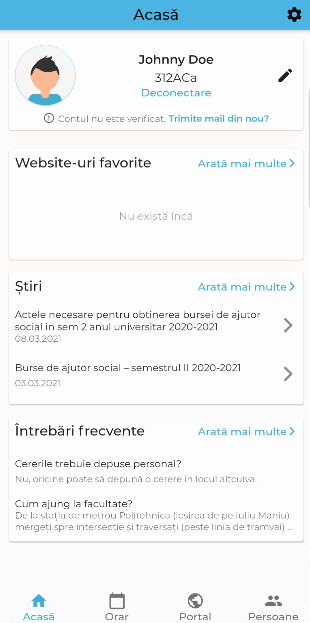
\includegraphics[width=\textwidth]{figures/beforedev/image10.png}
        \caption{Home page}
        \label{3:fig:homepage}
    \end{minipage}
    \hfill
    \begin{minipage}[b]{0.26\textwidth}
        \captionsetup{justification=centering}
        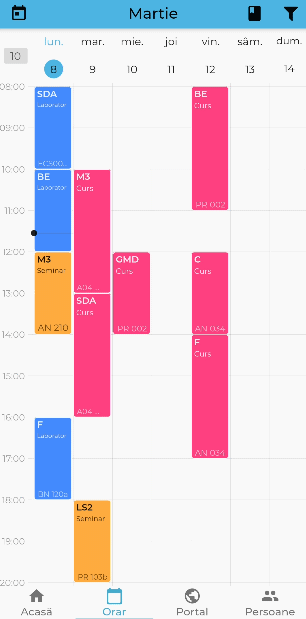
\includegraphics[width=\textwidth]{figures/beforedev/image2.png}
        \caption{Timetable page}
        \label{3:fig:timetable}
    \end{minipage}
    \hfill
    \begin{minipage}[b]{0.26\textwidth}
        \captionsetup{justification=centering}
        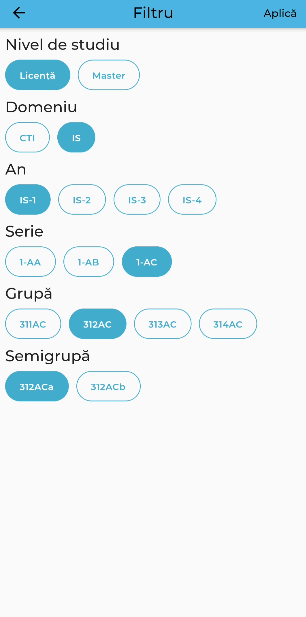
\includegraphics[width=\textwidth]{figures/beforedev/image20.png}
        \caption{Filter page}
        \label{3:fig:filter}
    \end{minipage}
\end{figure}

\begin{figure}[!ht]
    \centering
    \begin{minipage}[b]{0.26\textwidth}
        \captionsetup{justification=centering}
        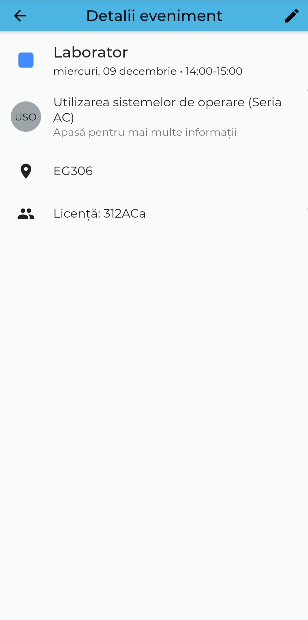
\includegraphics[width=\textwidth]{figures/beforedev/image19.png}
        \caption{Event details page}
        \label{3:fig:event}
    \end{minipage}
    \hfill
    \begin{minipage}[b]{0.26\textwidth}
        \captionsetup{justification=centering}
        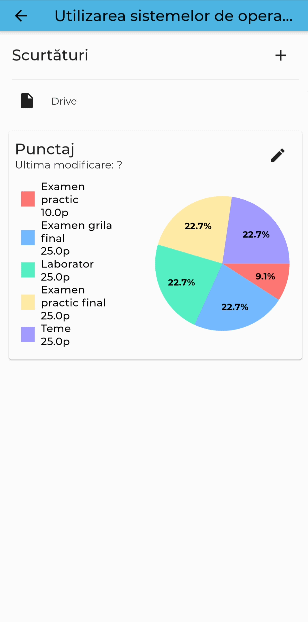
\includegraphics[width=\textwidth]{figures/beforedev/image4.png}
        \caption{Class details page}
        \label{3:fig:class}
    \end{minipage}
    
\end{figure}


As seen in figure \ref{3:fig:homepage}, the application’s home page contains elements are related to news, but lacks planning-related elements, leaving space for development that we will explore in the following chapters.

As we shift focus towards figure \ref{3:fig:timetable}, we find our main point of focus, namely the calendar page. We can see implemented simple and recurring events; both types also present inside Google’s Calendar.

~

The most significant advantage that ACS UPB Mobile brings is that by using a filter, like in figure \ref{3:fig:filter}, a user has instant access to his timetable without setting it up himself. This works because only one student has to introduce the events into the timetable, and these events propagate to those who choose to follow them. It is a simple and elegant solution to always having events updated for everyone, having just one person manage it. 

As we can further observe in figure \ref{3:fig:event}, when inspecting an event, it displays a list of information, such as the class linked to that event, time and date, location, and for whom it is addressed mainly, to aid the student. The course itself, shown in figure \ref{3:fig:class},  also has a representation as it is used to give a more comprehensive perspective. 

For our implementation, we need to just mention other existing features that we will be interacting with, as we are concerned with their functionalities rather than implementation: 
\begin{itemize}
            \setlength{\topsep}{0.5pt}
            \setlength{\itemsep}{0.5pt}
            \setlength{\parsep}{0.5pt}
            \item Users, as they are the main actor that interacts with all of the resources. We especially want to correlate users with timetable preferences without drastically changing their BLoC and data layer. 
           \item Filters, that mimic the structure of the ACS curricula and lets the users customize their interests. 
            \item Localization, as the application comes in different languages.
        \end{itemize}


\subsection{User engagement} \label{3:specificapp_engament}
Analyzing figure \ref{3:fig:firebase}, taken from the Firebase\footnote{https://firebase.google.com/} of ACS UPB Mobile, we can observe two big spikes around October in 2020 and March in 2021 that coincide with the beginning of each semester, giving us an insight into how the students use the app. We can presume that having a visual representation in the first weeks of each semester of the university schedule can significantly help memorize the events and not rely upon any calendar to optimize time management further.
\begin{figure}[ht]
    \centering
         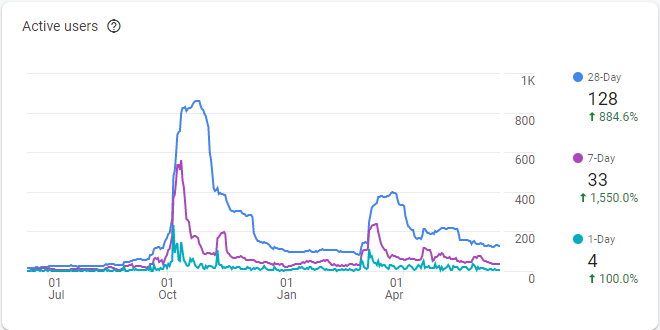
\includegraphics[width=0.95\textwidth]{figures/beforedev/image18.png}
    \caption{Active users} 
    \label{3:fig:firebase}
\end{figure}

~

While proving that the application is known among more than 800 different ACS students, these spikes are a starting point for the application’s success. 


\subsection{Conclusion} \label{3:specificapp_conclusion}
As presented in the anterior subsections, a specific application for handling scheduling university activities can gain spikes of users in short amounts of time. Furthermore, as the community based around the faculty is tightly bounded, ACS UPB Mobile can further increase its popularity. 

By adding a wide variety of productivity features and automating repetitive tasks, the spikes presented in the figure \ref{3:fig:firebase} provide a potential for retention, as users can freely experiment with the application and adopt it as a daily utility tool.

\section{Technology} \label{3:tech}

To properly understand the technicalities behind the application, we first need to describe the SDK used in the development process.

~

Flutter\footnote{https://flutter.dev/} is a Google open-source software development kit used to create user interfaces for cross-platform applications significantly faster. It is written in Dart\footnote{https://dart.dev/}, which is a programming language belonging also to Google.

To simply describe Dart, it resembles Java’s compilation process \cite{adl1998fast}, as it uses a Dart virtual machine, capable of just in time compilation, meaning the code can be updated as it runs, without having to stop and restart the application. In addition, it is object-oriented and supports both stateful and stateless components. 

Coming back to Flutter, the advantages of the programming languages translate into faster development, as compilation doesn’t stop the running process, and it also saves the state in unmodified components.
Flutter’s philosophy is writing code only one time and having it compiled and ran on any platform \cite{kuzmin2020experience}. This is possible because it doesn’t use any native components but instead uses the Skia graphic engine\footnote{https://skia.org/}. With this approach, the user can use an interface to create widgets, and the graphic engine handles the translation. 

Widgets are the conceptual building block of any Flutter application. They are versatile components used to create a visual interface. Together with the triggerable events, they compose the user interface and only deal with the application’s presentation layer. Therefore, widgets should only be a bridge between the users and the services.

~

This layered pattern is called BLoC, abbreviated from Business Logic Component \cite{flutter2020introduction}. It is a Three-tier architecture \cite{ibm2020arhi} that links the user interface to a controller layer that handles the logic and sends data to the model. 
The controller layer, also known as the BLoC layer, acts as a bidirectional channel and controls the separation of logic between conceptually different components. It is based on reactive programming and it is designed to work only with streams of data \cite{flutter2019bloc}. 

The last concept we will present is the state. As widgets can be of two types: Stateless and Stateful, we need to understand when to use one or the other:

-A Stateful widget is usually a dynamic component, suffering changes while the users interact with it. The state itself is a general mechanism for checking that the application behaves in predictable ways, even with unpredictable input.

-A Stateless widget is used in the opposite case, as the component doesn’t suffer any changes between renders. This doesn’t mean that the data never changes, but rather it is influenced by other processes triggers and it updates specifically when they occur. 

Like React\footnote{https://reactjs.org/}, Flutter has one advantage: its components are structured in a \textit{tree} form, with pages as the roots for integrating widgets. In addition, the widgets can incorporate other widgets, referred to as children. This arborescent structure is vital to the rendering mechanism, as when a branch changes, it only affects the elements on that branch, so much performance is gained by not heaving to re-render the whole tree \cite{muller2021web}. In this structure, it is recommended that Stateless Widgets are leafs, meaning nodes without any children, and have a Stateful parent, so when a change happens, it is propagated to the children and forces a render.


